\chapter{Secure Code Warrior}
\label{ch:scw}
\glsresetall

%CONTEXT
In the paved path methodology developers should be provided with deliberate, targeted education that keeps the developer experience in mind.
%NEED
This education should be \textit{relevant} to the developers work, \textit{efficient} in achieving their needs, and \textit{usable} to keep them engaged.

%TASK/OBJECT
In this chapter I describe the education provided by the online learning platform created by \gls{scw}. 
I assess its potential for use in the paved path methodology and describe shortcomings that require further research.


\summarybox{
%FINDINGS
The \gls{scw} training platform provides training to hundreds of thousands of developers from reputable customers.
It provides defensive exercises in a gamified and engaging way and offers a wide variety of programming languages and frameworks. 
%CONCLUSION
It is suitable to be used in the paved path methodology as it is \textit{relevant} and \textit{usable}.
However, there is room for improvement when it comes to the \textit{efficiency} of the training.
All users, regardless of skill level, are presented challenges of the same difficulty.
This leads to boredom or frustration for some users and might cause them to disengage from the training.}

\section{The company}
The company was co-founded by Pieter Danhieux and Matias Madou Ph.D., two alumni of Ghent University and both globally recognized security experts.
During their international careers both founders noticed that the focus in industry is too often on remediation rather than prevention of \glspl{security problem} in software.
Their vision is not to make a security expert out of every developer, but to empower them to become the first line of defence in the organisation.
The company provides education and tools to improve secure coding skills of developers.
Both the online training platform and their IDE based security tool can be deployed to support a paved path methodology as described in this book.

Since its start in 2015, more than 240 customers from 32 countries around the world use \gls{scw} products to improve the secure coding skills within their development teams.
\Gls{scw} focuses on large companies with lots of developers. Most customers are active in banking, finance, government, aviation, or telecommunications. Some notable customers are:

\begin{itemize}
\setlength\itemsep{0em}
    \item Coupang: the largest online retailer in South Korea
    \item 19 of the top 100 global banks
    \item \gls{bbc}: the largest broadcaster in the world
    \item 2 of the world's largest telecommunications providers
    \item 2 of the top US credit card processors
    \item Zoom: one of the largest communication technology companies
\end{itemize}

\section{The training platform}

The training platform provides an interactive and gamified way to learn secure coding concepts, and focuses on defensive techniques. 
In the mission control dashboard, shown in Figure~\ref{fig:mission}, developers are tasked with defending an application from different types of threats originating from all over the world.
The developer is awarded points for completing exercises, and leaderboards are shown to create a competitive environment.
By collecting enough points and spending enough time on the platform the developer can unlock achievements and gain badges.
All of this progress can be monitored on a metrics dashboard, shown in Figure~\ref{fig:metrics}.
A total of over 100,000 unique developers used the training platform in 2020.

In a survey with 722 developers, 90\% of respondents said they prefer \gls{scw} over traditional classroom learning
and 85\% prefer it over other online learning resources they have tried in the past.
These results are also confirmed by many testimonies, such as the following response on TechValidate\footnote{\url{techvalidate.com/product-research/secure-code-warrior/facts}}. 

\begin{displayquote}
Secure Code Warrior’s use of gamification has helped us emphasize the importance of secure coding in a refreshingly fun and engaging way. \textit{-- Developer at Global 500 Financial Services Company}
\end{displayquote}

\begin{sidewaysfigure}
  \centering
  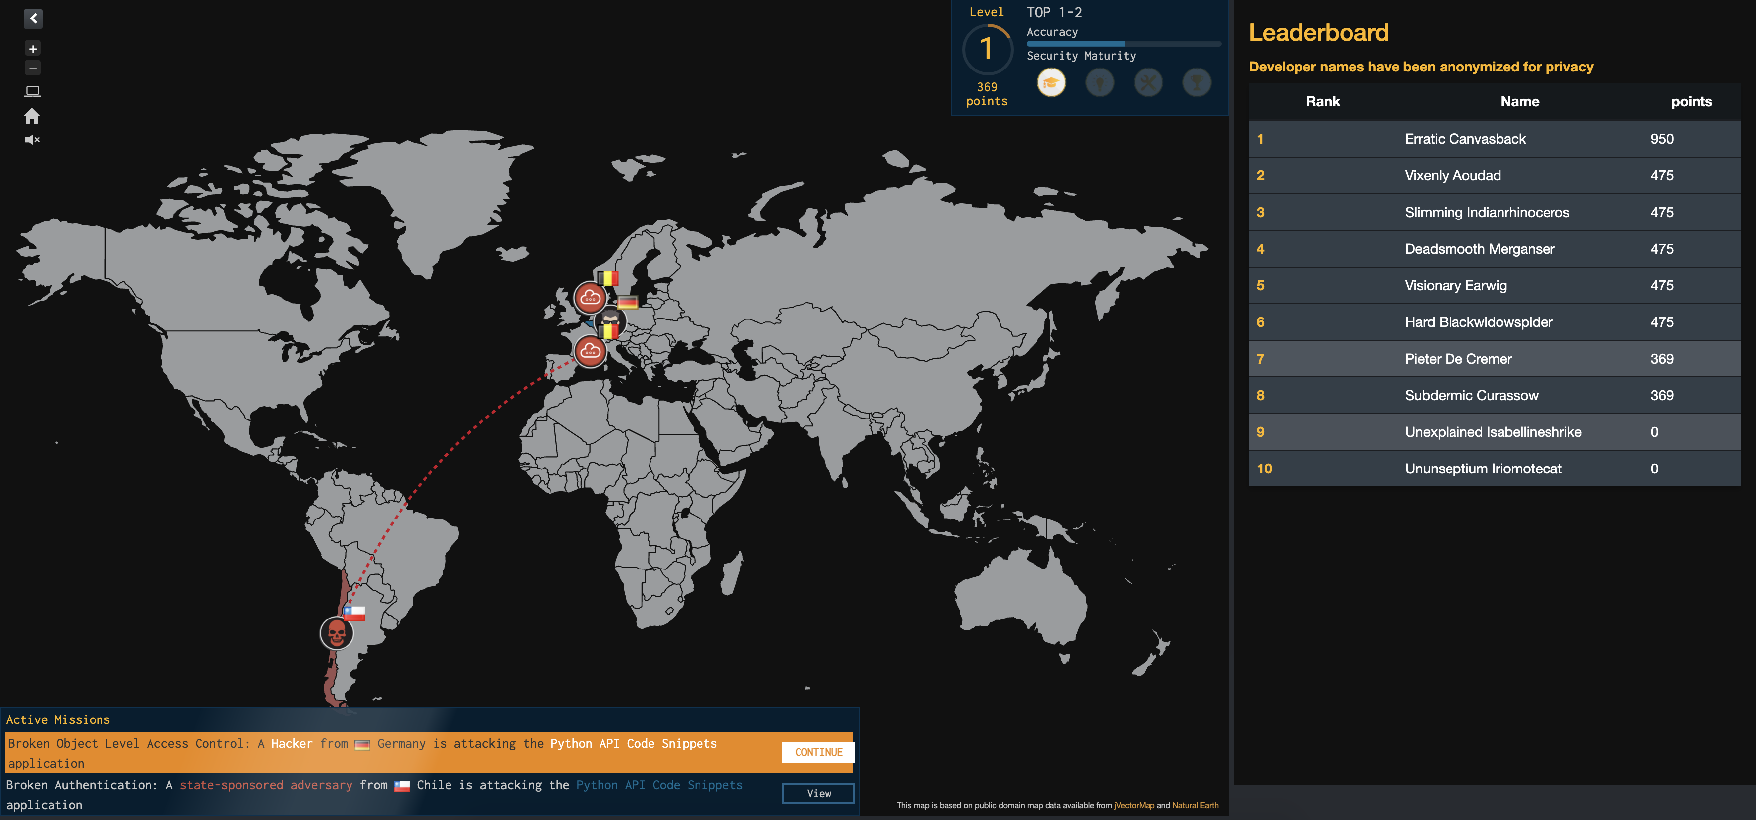
\includegraphics[width=\textwidth]{mission.pdf}
  \caption[SCW mission control dashboard]{The mission control dashboard on the \gls{scw} platform creates a gamified overview of the exercises.}
  \label{fig:mission} 
\end{sidewaysfigure}

\begin{sidewaysfigure}
  \centering
  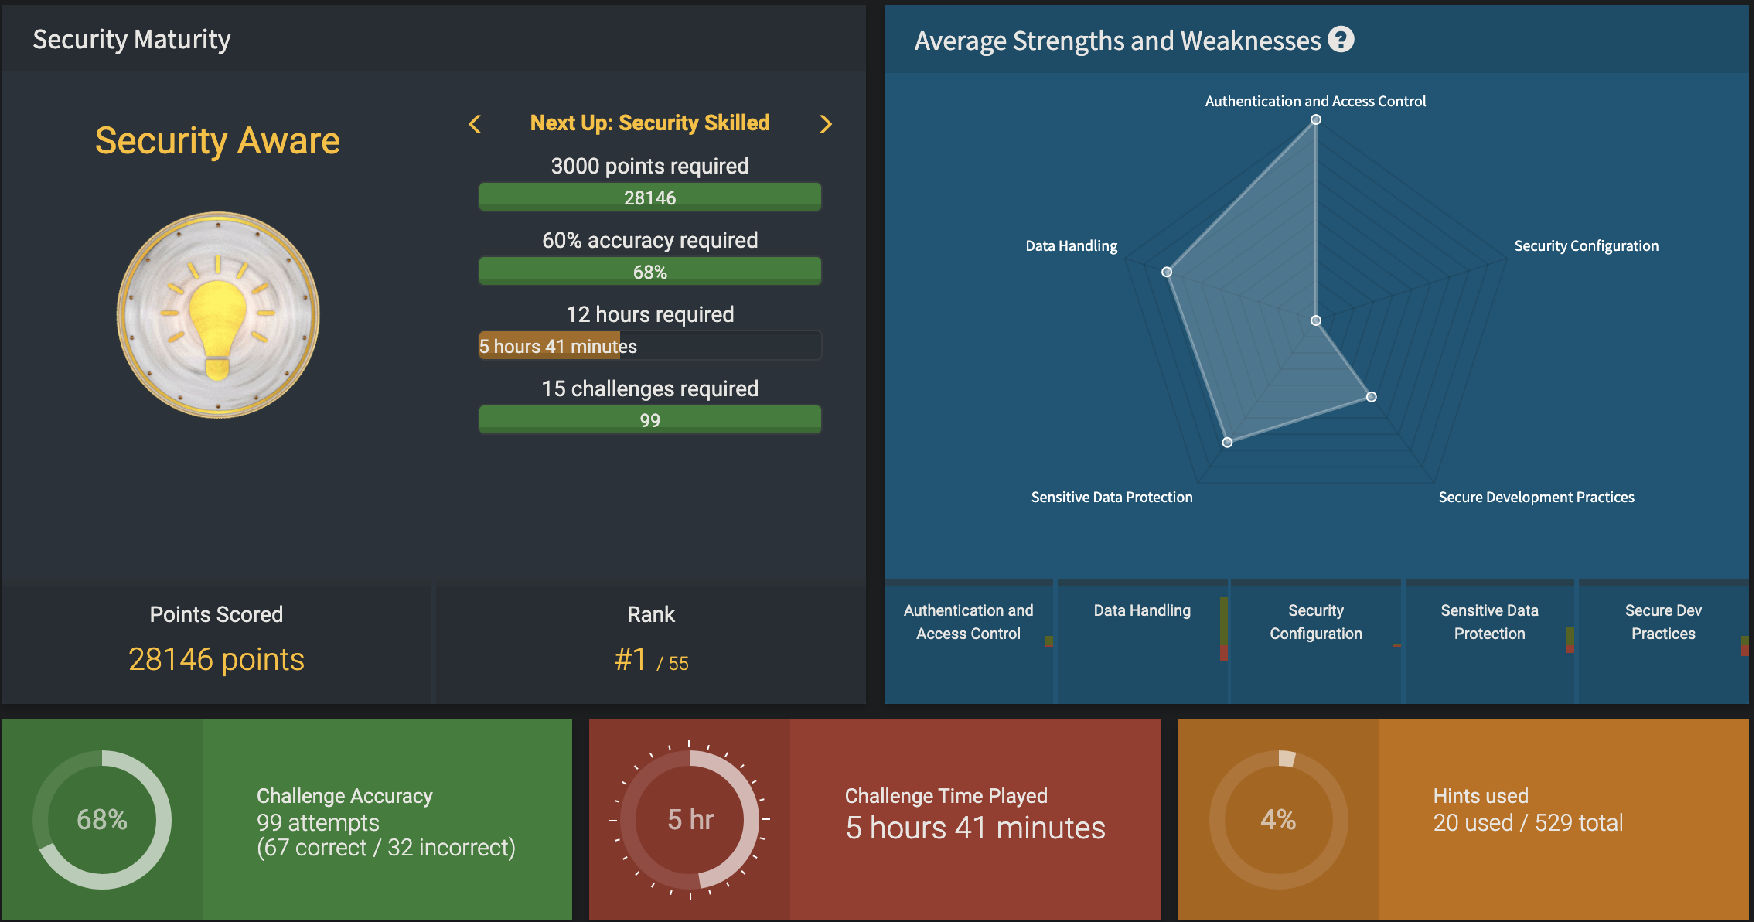
\includegraphics[width=\textwidth]{metrics.pdf}
  \caption[SCW metrics dashboard]{The metrics dashboard on the \gls{scw} platform allows developers to monitor their progress and unlock new badges.}
  \label{fig:metrics} 
\end{sidewaysfigure}

\section{Exercises}
\label{sec:challenges}
Training exercises on the \gls{scw} platform, often called challenges, are most frequently created from a complete and secure software application such as a webstore or a banking application. To create a challenge, a \gls{vulnerability} is introduced into this application on purpose.
The challenge is presented to the users as one of three types of exercises, each assigned a numerical level, an \textit{identify} (L1), \textit{locate} (L2), or \textit{fix} exercise (L3).

Identify exercises (L1) mark the insecure code fragment and provide the developer with a number of \gls{vulnerability} categories. It is up to the developer to identify which of the provided categories best describes the vulnerability present in the code fragment. In Figure~\ref{fig:identify} an identify exercise is shown based on a \gls{sql} injection in a Python web application.

For locate exercises (L2), the category of the vulnerability that is present in the insecure code fragment is given.
The insecure code fragment is marked, as well as several other (secure) code fragments. 
It is up to the developer to locate which code fragment contains the insecurity.
An example of a locate exercise is shown in Figure~\ref{fig:locate} using the same \gls{sql} injection in the same Python web application as the identify exercise in Figure~\ref{fig:identify}.

Fix exercises (L3) show both the insecure code fragment and the category of the inserted vulnerability to the user. 
Four alternatives are shown, with changes made to the insecure code fragment, and sometimes to other parts of the application code as well.
The developer needs to find the most secure alternative among the four options.
A fix exercise is shown in Figure~\ref{fig:fix}, again using the same \gls{sql} injection as before. 
Fix (L3) exercises are often combined with identify (L1) or locate (L2) exercises. 
These challenges then consist of two stages, in the first stage the vulnerability needs to be identified or located, in the second stage the exact same vulnerability needs to be fixed. 
The resulting two-stage challenge is an identify-and-fix (L4 = L1 + L3) or a locate-and-fix (L5 = L2 + L3) challenge.

%\begin{figure}
%\centering
%\begin{subfigure}[b]{\textwidth}
%\sidebysidecaption{0.05\linewidth}{0.95\linewidth}{
%   \caption{}
%   \label{fig:identify}}{
%   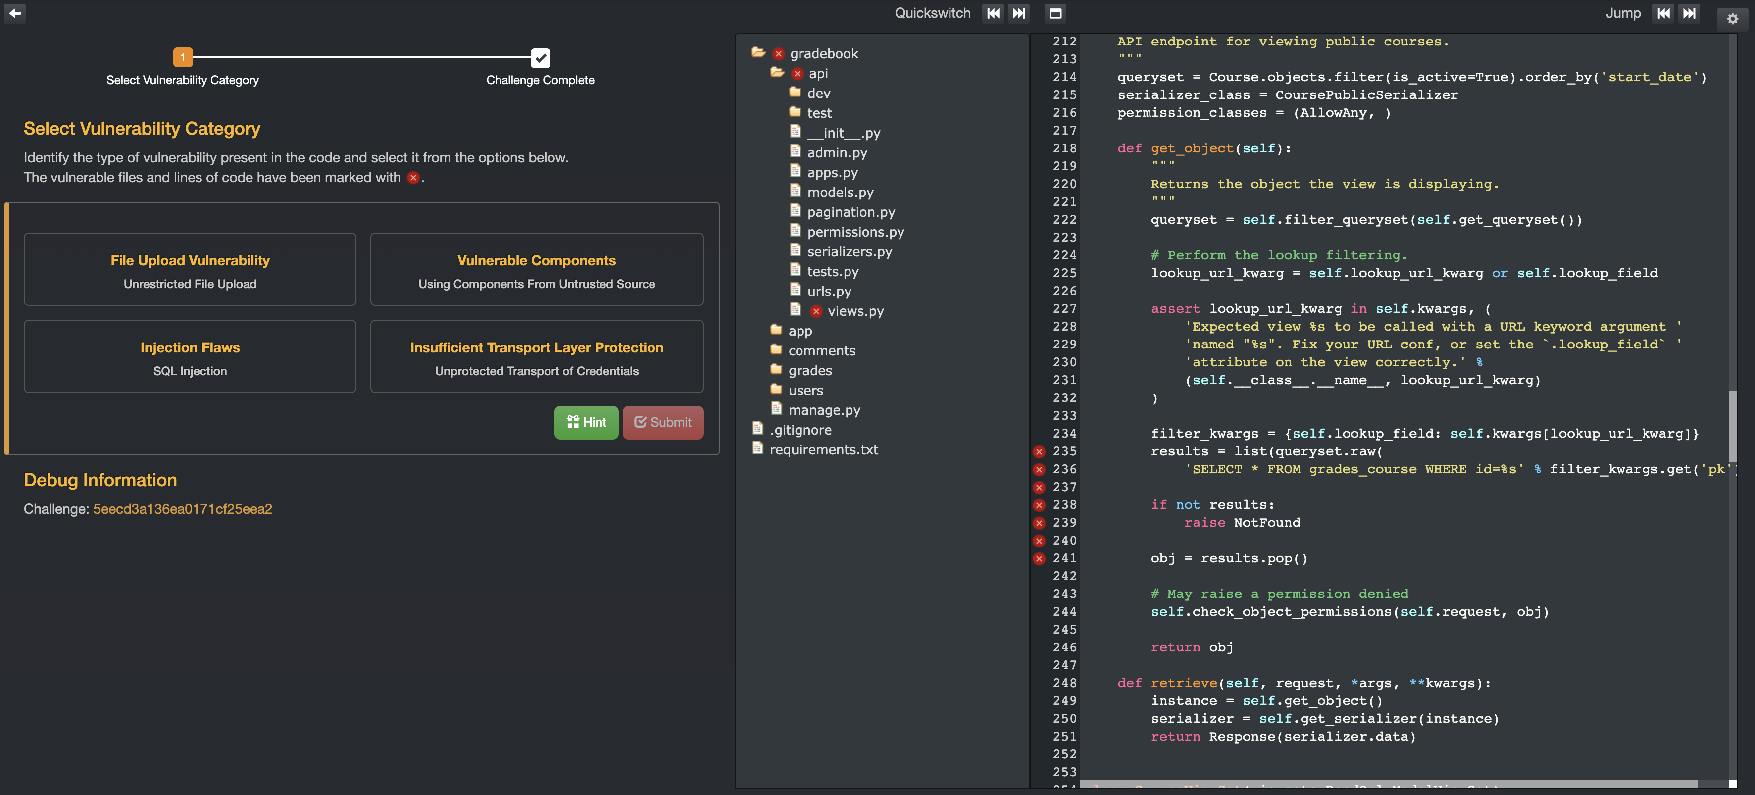
\includegraphics[width=0.95\linewidth]{identify.pdf}}
%\end{subfigure}
%
%\begin{subfigure}[b]{\textwidth}
%\sidebysidecaption{0.05\linewidth}{0.95\linewidth}{
%   \caption{}
%   \label{fig:locate}}{
%   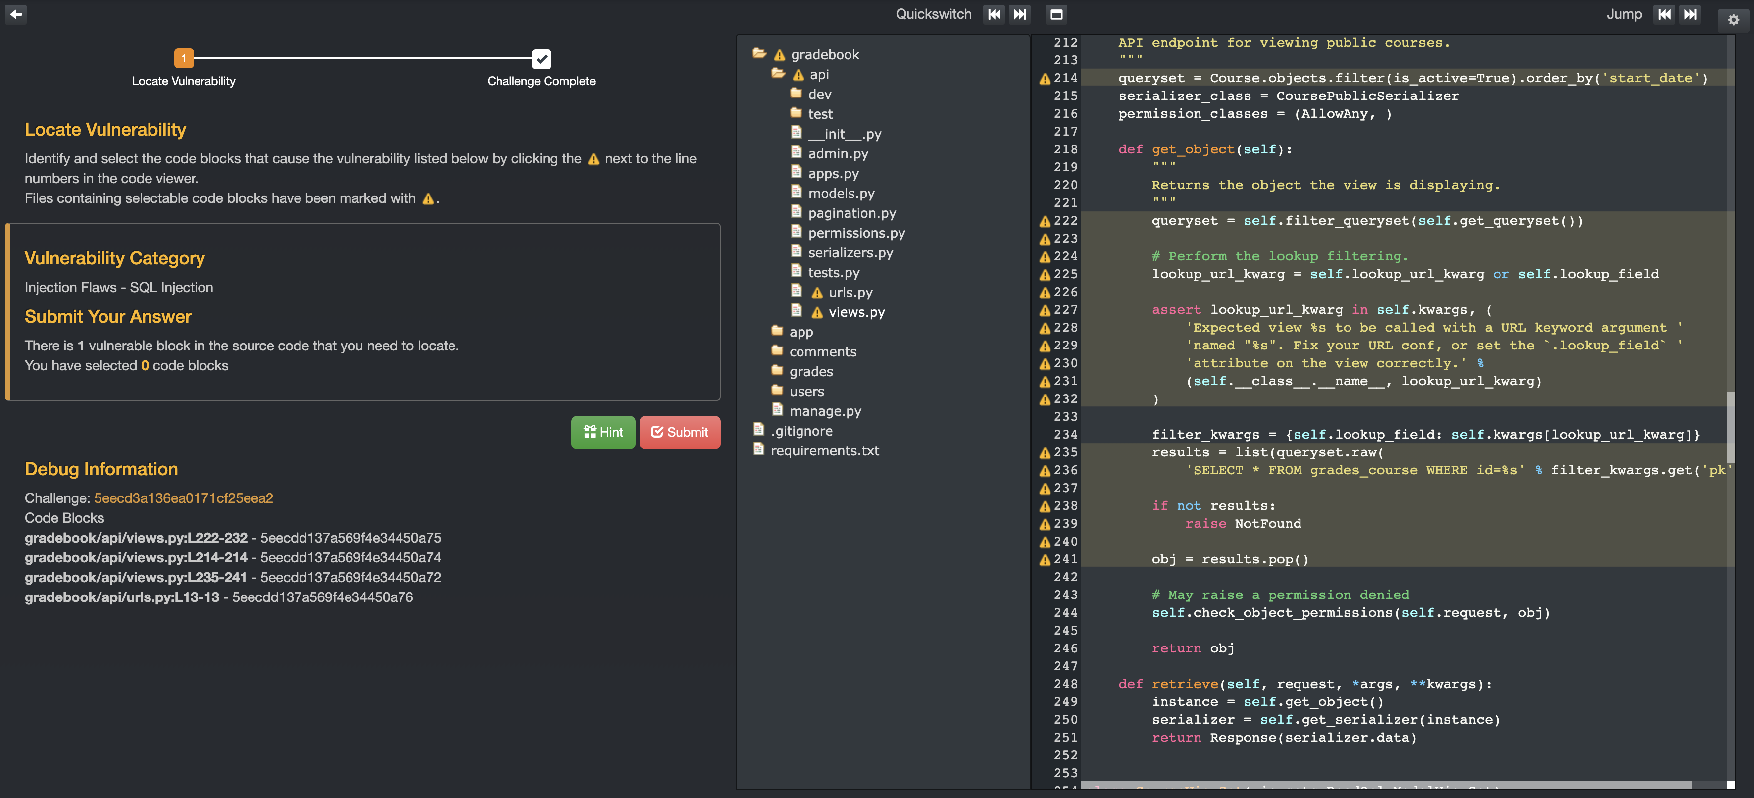
\includegraphics[width=0.95\linewidth]{locate.pdf}}
%\end{subfigure}
%
%\begin{subfigure}[b]{\textwidth}
%\sidebysidecaption{0.05\linewidth}{0.95\linewidth}{
%   \caption{}
%   \label{fig:fix}}{
%   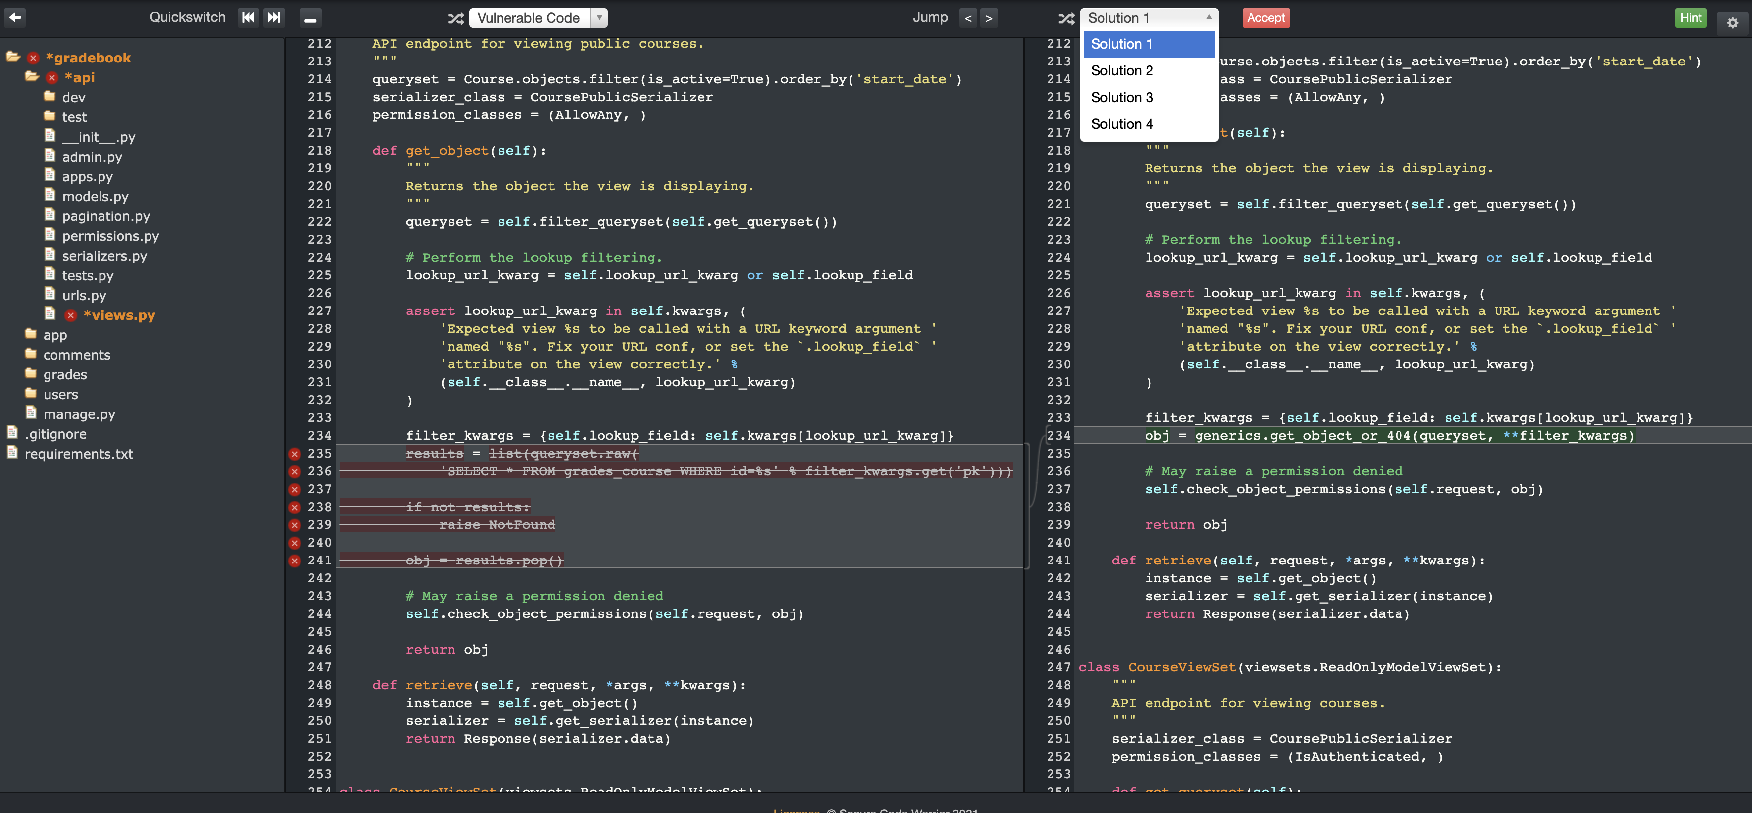
\includegraphics[width=0.95\linewidth]{fix.pdf}}
%\end{subfigure}
%
%\caption[Locate, identify, and fix challenges]{A single vulnerability in a software application can be presented to the developer as three different challenge types. \textit{Identify} exercises (a) mark the vulnerable code fragment and require the developer to select the right category. \textit{Locate} exercises (b) present the vulnerability category and require the developer to select the code fragment containing this vulnerability. \textit{Fix} exercises (c) require the developer to find the secure option among four alternative code bases.}
%\end{figure}

\begin{sidewaysfigure}
  \centering
  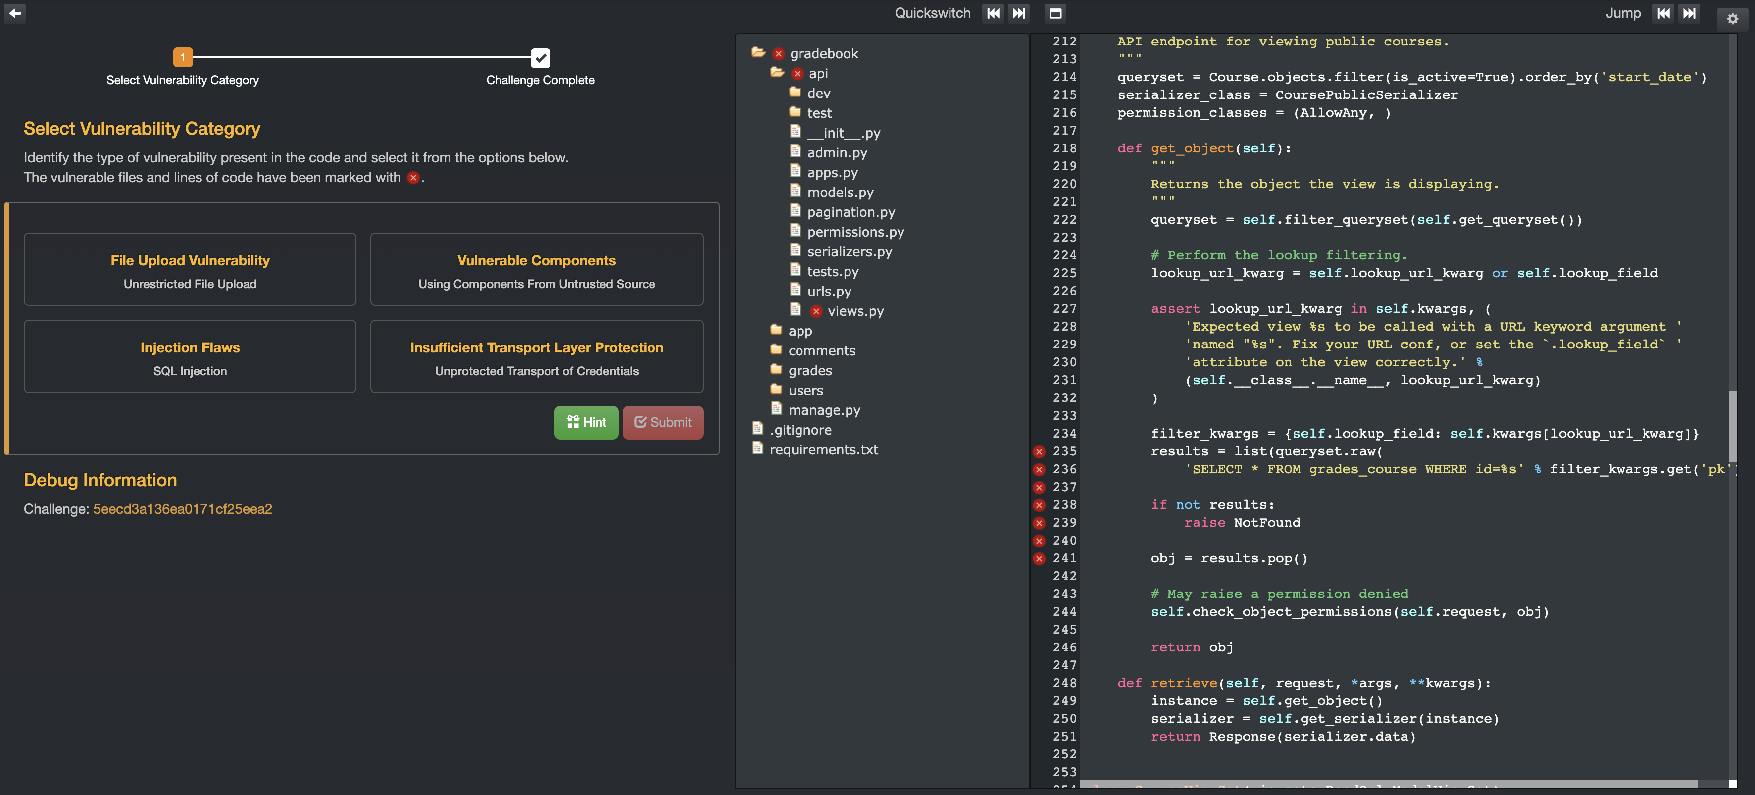
\includegraphics[width=\textwidth]{identify.pdf}
  \caption[Identify challenge]{\Gls{sql} injection in a Python web application presented as an identify exercise, the first of three different challenge types on the \gls{scw} platform.}
  \label{fig:identify} 
\end{sidewaysfigure}

\begin{sidewaysfigure}
  \centering
  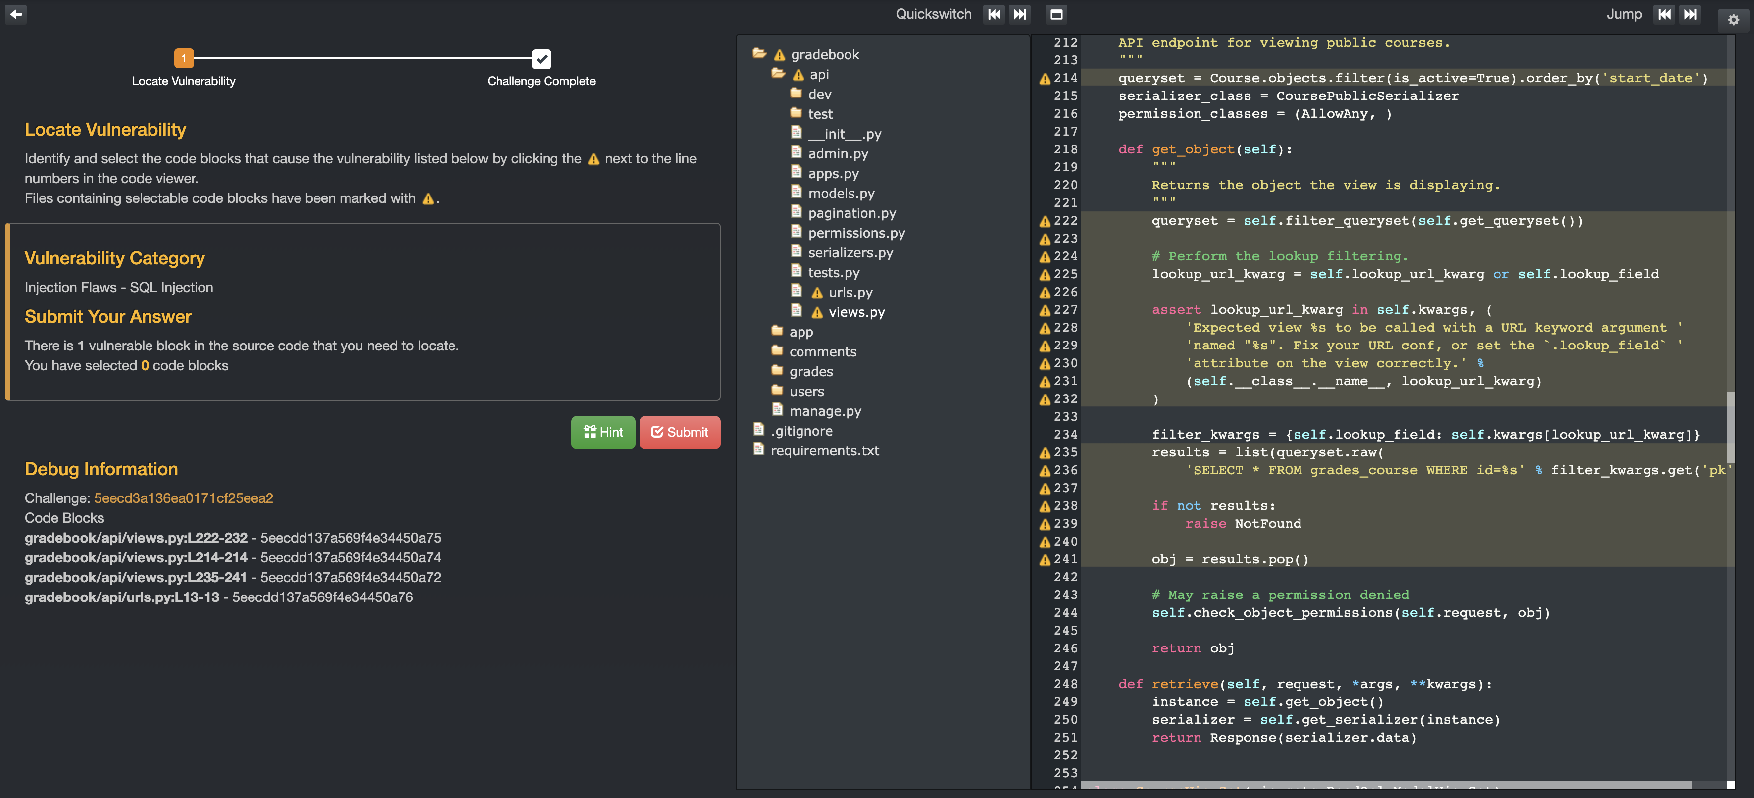
\includegraphics[width=\textwidth]{locate.pdf}
  \caption[Locate challenge]{\Gls{sql} injection in a Python web application presented as a locate exercise, the second of three different challenge types on the \gls{scw} platform.}
  \label{fig:locate} 
\end{sidewaysfigure}

\begin{sidewaysfigure}
  \centering
  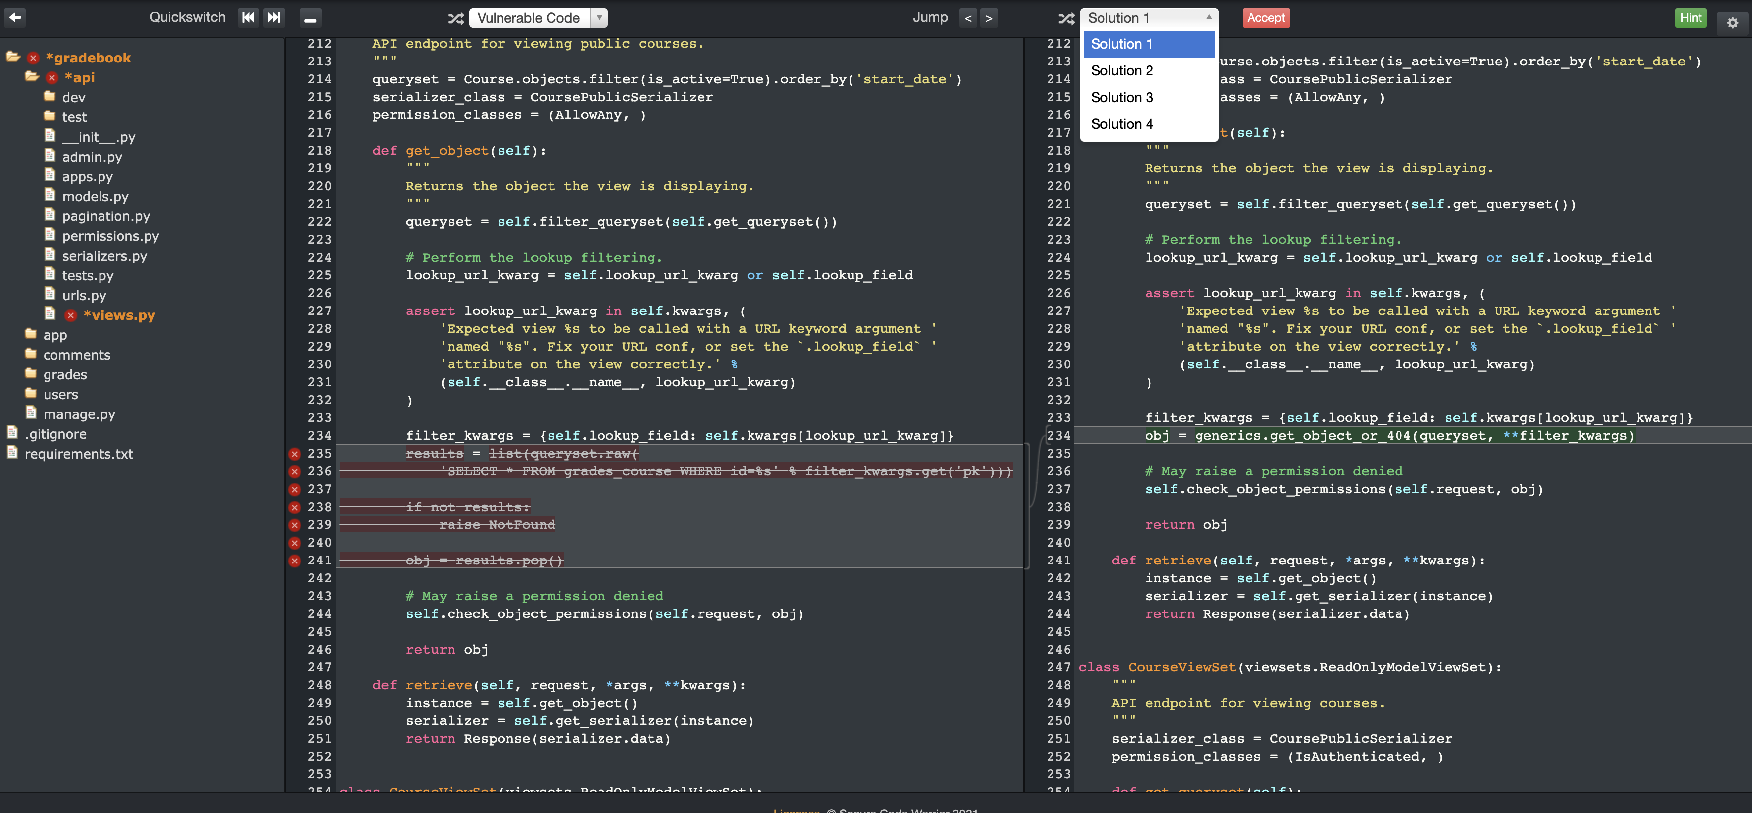
\includegraphics[width=\textwidth]{fix.pdf}
  \caption[Fix challenge]{\Gls{sql} injection in a Python web application presented as a fix exercise, the thrid of three different challenge types on the \gls{scw} platform.}
  \label{fig:fix} 
\end{sidewaysfigure}

Recently new and more interactive challenge types are being developed. 
One such type requires the developer to construct input that successfully exploits the vulnerability present in the application. 

\section{Context}
The challenges are presented to users in different contexts, these are training mode, tournament mode, or assessment mode.

The default context is the training mode, in this mode the developer is allowed to use as many hints as needed.
They are also allowed an unlimited amount of attempts to find the right answer.
Each hint or failed attempt reduces the amount of points that the developer is awarded.
Appendix~\ref{app:challenges} describes in more detail how the difficulty of a challenge, the amount of hints used, and the number of failed attempts determine how many points are awarded. 
Developers are free to choose which challenges they solve first in training.
A standard course is provided that guides them through the \gls{owasp} Top 10 categories and many developers complete this course before trying other challenges.

In tournament mode the scoring method and availability of hints and attempts can be adjusted by the host.
In this mode, all participants are shown exercises about the same vulnerability type and of the same difficulty but in their language of choice.
The tournament is run for a limited time, usually a few hours, in which the contestants can complete the challenges.
In tournament mode a live leaderboard is visible that can optionally be hidden close to the end for suspense.
Since all participants are shown the same number of exercises having the same difficulty, it often comes down to speed to finish the challenges in time, and accuracy to lose as few points as possible through hints or mistakes.

In assessment mode no hints are available and only one attempt is allowed for each challenge. This mode is used to evaluate the performance of a user.
Customers can select the vulnerability type and difficulty of the challenges making up the assessment.
There are some templates provided as an example that test for knowledge of the \gls{owasp} Top 10.

\section{Course material}
The \gls{scw} training portal provides training in more than 50 languages and frameworks\footnote{\url{https://www.securecodewarrior.com/supported-languages}}, ranging from Cobol to Go, including languages for web, mobile, cloud, and embedded software.
The training content covers 184 different vulnerability types, including those in widely-used lists such as the \gls{owasp} Top 10\footnote{\url{https://owasp.org/www-project-top-ten/}}, \gls{owasp} Top 10 Mobile, \gls{owasp} Top 10 \gls{api} Security and the \gls{cwe} Top 25\footnote{\url{https://cwe.mitre.org/top25}}.
The full list of vulnerabilities can be found on the \gls{scw} website\footnote{\url{https://www.securecodewarrior.com/product/supported-vulnerabilities}}.
This coverage is not homogeneous across all languages.
For each language and framework, each relevant vulnerability type is assigned a priority (high, medium, or low).
This priority depends on the severity and prevalence of the vulnerability type in this particular language and framework combination.

How well a language is covered then depends on the amount of challenges that covers vulnerability types of different priorities. 
The minimum requirement for a language to be considered ready for training is three challenges for each category in the \gls{owasp} Top 10 categories.
A language is considered tournament ready when there are five challenges (two easy, two medium and one high difficulty) for all vulnerability types with high priority, and two challenges (one easy, one medium) for all vulnerability types with medium priority.
There are other requirements still for assessments, specific courses, or the website trial.

For each of the top three frameworks over 450 unique vulnerabilities have been introduced in applications. These frameworks are C\# \gls{mvc} (461 vulnerabilities), Java \gls{ee} \gls{jsp} (475 vulnerabilities), and Java \gls{ee} Spring (495 vulnerabilities). When multiplied by three (for identify, locate, and fix), there are over 1350 challenges for each of these three frameworks.

\section{Use in the paved path methodology}
The \gls{scw} online learning platform is a great educational resource to support the paved path methodology.
The platform is \textit{relevant}, the learning context resembles the developer's work context as they are able to receive training in their office or home office and by looking at actual code. 
The code on the platform is likely to be similar to that of the developer due to the wide variety of programming languages, frameworks, and software types that are supported. 
The exercises teach a developer a secure paved path in their framework of choice. The identify, locate, and fix exercises are all defensive tasks created with the developer in mind.

The platform is also \textit{usable} as there are several features to increase interactivity and engagement, such as the gamified theme, leaderboards, tournaments, achievements, and badges.
A structured journey is present in the form of courses, such as the \gls{owasp} Top 10 courses.
The learning material is presented through multiple choice questions, and in the newly developed exercises that will be released in the future developers will even be allowed to discover the answer through trial and error instead of picking from a list of options.

% the NEED
There is certainly enough content available to allow for sufficient repetition so that the concepts can be committed to memory, with some frameworks providing as many as 1350 challenges.
However, there is no guidance to find the right balance between repetition and \textit{efficiency}.
The exercises often do not match the learning pace of each individual, leading to boredom or frustration.
This is apparent from the challenge completion rate, as only 45\% of users complete more than 30 challenges, the amount of challenges in an \gls{owasp} top 10 course.

When surveyed, some users indicate this possible mismatch in the learning pace.
More than 700 respondents were asked to describe their experience using the \gls{scw} portal after completing a tournament.
To do this they were able to choose words from a set of options or write their own.
Many respondents selected words indicating their engagement such as interactive (55\%), engaging (53\%), and fun (48\%).
But some also picked words that could indicate an incorrect learning pace, among which challenging (45\%), repetitive (21\%), long (7\%), and boring (4\%).
Only 22 (3\%) respondents wrote down additional words themselves, some of which indicate mismatches in learning pace. 
Two users wrote down tedious, two users wrote cumbersome, one wrote frustrating, and one even went as far as to describe their experience as gambling.

In conclusion, the \gls{scw} online learning platform is a good educational resource when using a paved path methodology. Its defensive exercises and wide support for different programming languages and frameworks make it \textit{relevant} to the developer's work. The gamification and interactivity keep it \textit{usable} and fun. However, when it comes to the \textit{efficiency} of the training there is still room for improvement as currently all users are presented with challenges of the same difficulty regardless of their skill level and learning pace. User feedback indicates that this leads to boredom or frustration for some of the users. 